% !TEX root = ../main.tex

\chapter{通道级特征再学习方法提取精细支气管特征}\label{chap:feature_relearning}

在前文3D-UNet网络基准模型分割出的支气管气道树的基础上,仔细观察表\ref{tbl:visualize_airway_3d_model}和表\ref{tbl:3dunetad_airway_tree}
里的支气管三维气道树,一个普遍的规律是:在气管Trachea(第0代)、左右主支气管Left/Right main bronchi(第1代)、
上/中/下叶支气管Superior/Middle/Inferior lobar bronchus(第2代)这三代支气管上分割良好,但在段支气管Segmental bronchi(第3代)分割上
出现很多绿色假阳性或红色假阴性体素,而到了小叶支气管Lobular bronchi(第4代)的分割上出现了大量的断裂,最后的细支气管Bronchiole(第5代,连接到最终的肺泡)
因为太小而完全没有标注,所以在分割的三维气道树上不存在。对于采用了同样的卷积层和池化层来说,第0代/第1代/第2代的支气管分割效果明显比第3代/第4代的支气管要好得多。
考虑到3D-UNet网络是将切割成$D90 \times H192 \times W304$大小的长方体数据作为最小输入单元的。就以标注数据来说,相同体积的切割体1与2(见图
\ref{fig:voxel_density_diffs})
\begin{figure}[h]
    \centering
    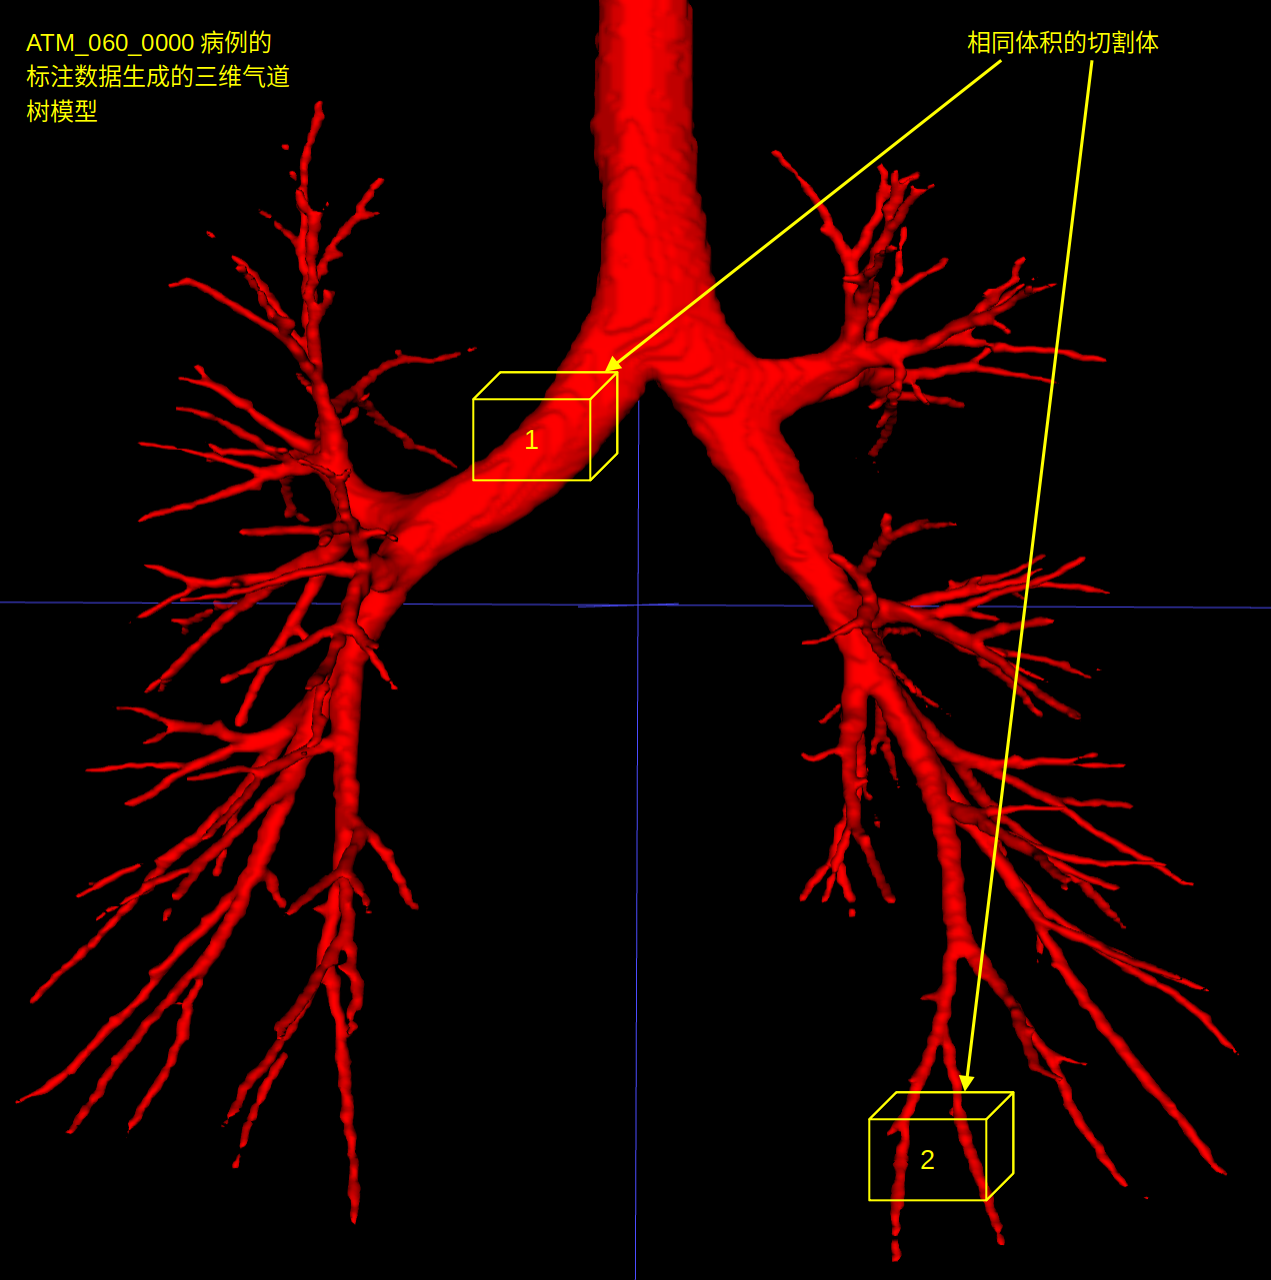
\includegraphics[width=0.6\textwidth]{相同体积的切割体}
    \bicaption[相同体积的切割体在不同空间位置获得的体素密度差异]
        {相同体积的切割体在不同空间位置获得的体素密度差异}
        {The voxel density difference under different spatial location}
    \label{fig:voxel_density_diffs}
\end{figure}
在不同的空间位置,它们所容纳的支气管体素密度差异巨大。这个最小输入单元经过卷积层和池化层,空间分辨率会降低一半。若采用平均池化的方法,切割体2处的精细
特征可能会被“擦除掉”,而切割体1处的粗糙特征还能保留下来。即使采用最大池化方法,经过多层卷积和池化后,精细特征也会逐渐消失。因此,我们认为在当前特征和
分辨率尺度内,不同的空间位置有不同的重要性。尤其像支气管这样的树状结构,要想获得精细的高代支气管特征,显然需要提高它们的重要性,也就是它们的权重。
为了解决这个问题,我们提出一种通道级特征再学习(Channel-wise feature re-learning)方法,拟在卷积层块之后、最大池化层(见图\ref{fig:convblock})之前
添加一个通道级特征再学习模块来进行再校准,捕获更精细的特征。

\section{通道级特征再学习方法}
下面来说明通道级特征再学习方法的基本原理。

给定一个肺部支气管CT扫描图像体$\mathbbm{X}_{airway}$,则我们的支气管气道树分割任务可描述为式\ref{eq:seg_function}的函数关系,
\begin{align}\label{eq:seg_function}
    \mathbbm{Prob}_\mathit{airway} = \mathscr{F}\left( \mathbbm{X}_\mathit{airway} \right)
    \shortintertext{s.t.}
    \min \Bigm|\mathbbm{Prob}_\mathit{airway} - \mathbbm{GT}_\mathit{airway}\Bigm|
\end{align}
其中$\mathbbm{Prob}_\mathit{airway}$表示气道的预测概率。我们做支气管气道树分割的目标是通过3D-UNet网络学习到一个端到端的映射函数$\mathscr{F}$,使得
预测值$\mathbbm{Prob}_\mathit{airway}$与真实值$\mathbbm{GT}_\mathit{airway}$之差最小化。

3D-UNet网络的最小输入单元是一个三维(立方)体数据,在第$m$个卷积层块的特征输出$\mathbbm{Feat}_m$表示为一个$C_m \times D_m \times H_m \times W_m$大小的四维矩阵
$\mathbbm{Matrix}_{C_m \times D_m \times H_m \times W_m}$,即表示有$C_m$个大小为$D_m \times H_m \times W_m$的立方体。当$m = 1$时,即
第一个卷积层块输出的特征含有16个大小为$D80 \times H192 \times W304$的立方体,这个立方体就是图\ref{fig:voxel_density_diffs}的一个切割体。
如图\ref{fig:feature_dimensions}所示。
\begin{figure}[h]
    \centering
    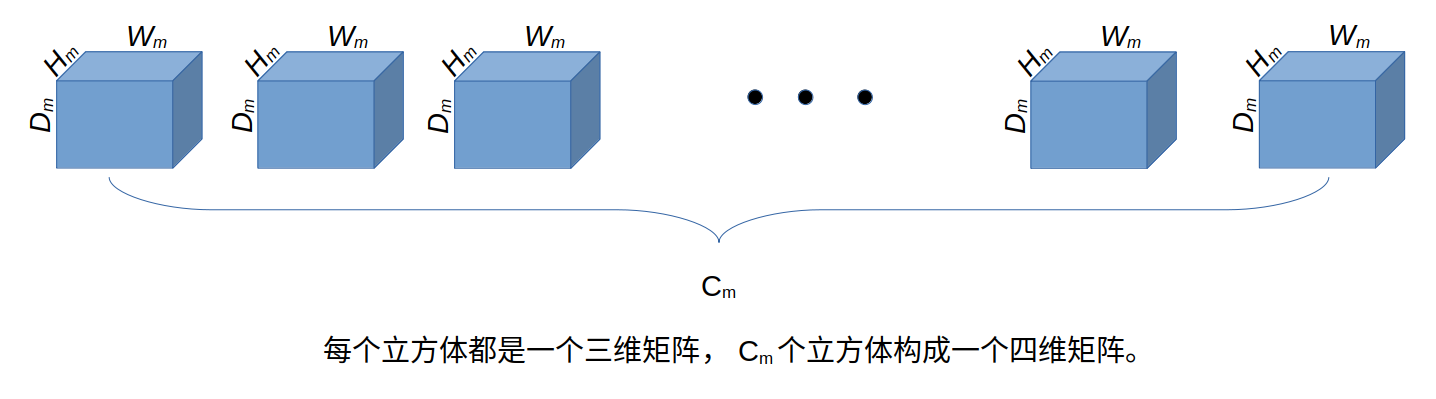
\includegraphics[width=0.7\textwidth]{特征的维数}
    \bicaption[卷积层块的特征的维数]
        {卷积层块的特征的维数}
        {The dimensions of feature output from convolutional block layer}
    \label{fig:feature_dimensions}
\end{figure}
其中,$C_m$、$D_m$、$H_m$和$W_m$分别表示通道维(Channel)、深度维(Depth)、高度维(Height)和宽度维(Width)。借用PyTorch的张量表示法,
则$\mathbbm{Feat}_m$中的任意元素
\begin{equation}\label{eq:feature_dimensions}
    \mathbbm{Feat}_m[c, d, h, w] \in \mathbbm{Matrix}_{C_m \times D_m \times H_m \times W_m}
\end{equation}
其中$c, d, h, w$分别指的是通道维、深度维、高度维、宽度维的索引号。

我们要构建的特征再学习就是要定义一个对当前卷积层特征$\mathbbm{Feat}_m$的通道算子$\varPsi$。那么对应的特征再学习(Feature Re-Learning, FRL)可定义为函数关系:
\begin{equation}
    \mathbbm{FRL}_m = \varPsi\left(\mathbbm{Feat}_m\right)
\end{equation}
特征再学习的通道算子是为了校准卷积层特征输出,它是一个通道级的权重图,不仅仅可以识别特征$\mathbbm{Feat}_m$的关键空间位置的信息,譬如图\ref{fig:feature_dimensions}
切割体1所在位置的粗大枝干的粗糙特征和切割体2所在位置的末梢枝节的精细特征,还可以加强影响输出决策的基本通道。我们采用沿着每个空间维度(深度维、高度维、宽度维)的特征加权
(通道)组合的方式来集成空间位置的信息。 这是一种空间积分的方法,也称为体积分,如\ref{eq:spatial_integration}式对第$m$个卷积层输出特征$\mathbbm{Feat}_m$
的体积分$\int_{V}\mathbbm{Feat}_m\dd V$。
\begin{equation}\label{eq:spatial_integration}
\begin{split}
    \varPsi\left(\mathbbm{Feat}_m\right) &= \int_{V}\mathbbm{Feat}_m\dd V \\
                                         &= \int_{V}\mathbbm{Feat}_m\dd (\mathit{Depth}) \\
                                         &+ \int_{V}\mathbbm{Feat}_m\dd (\mathit{Height}) \\
                                         &+ \int_{V}\mathbbm{Feat}_m\dd (\mathit{Width})
\end{split}
\end{equation}
我们把这种体积分拆成分别沿深度、高度和宽度3个轴方向的积分之和。为了阐述这种体积分是如何进行的,我们从图\ref{fig:feature_dimensions}取出一个立方体来
对照着讲解。如图\ref{fig:spatial_integration}所示,
\begin{figure}[!htp]
    \centering
    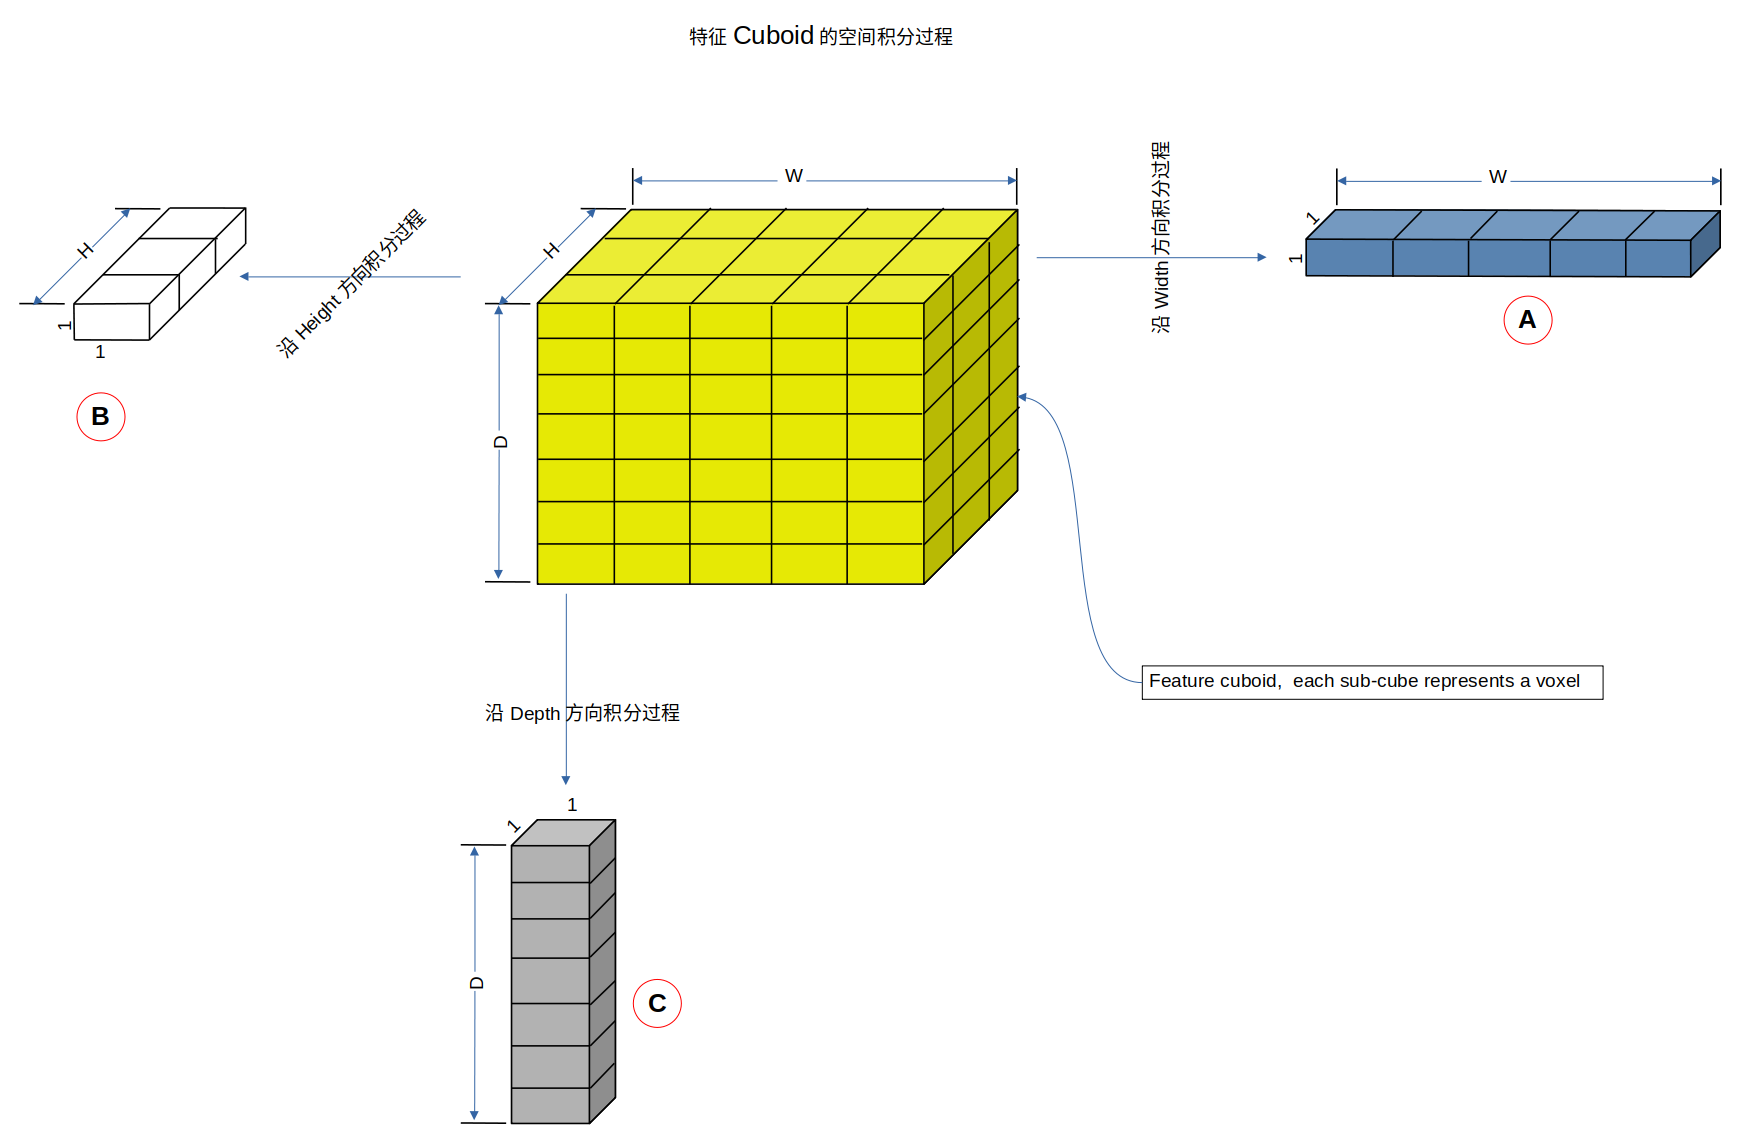
\includegraphics[width=\textwidth]{feature_cuboid_spatial_integration}
    \bicaption[特征立方体的空间积分过程示意图]
        {特征立方体的空间积分过程示意图}
        {The spatial integration process for feature cuboid}
    \label{fig:spatial_integration}
\end{figure}
特征立方体的大小为$D \times H \times W$\footnote{本文在描述特征的维数或者张量的Shape时,统一按照PyTorch对张量的维数从高到低依次为: 批次维Batch、通道维Channel、
深度维Depth、高度维Height、宽度维Width。简写取首字母[B, C, D, H, W],全文都采取这样的方式描述。},每一个小立方体的大小是$1 \times 1 \times 1$,表示为一个体素。

沿$Width$方向的积分$\int_{V} \mathbbm{Feat}_m \dd (\mathit{Width})$过程实际上是将$D \times H \times W$的特征立方体挤压成$1 \times 1 \times W$的形状(
图\ref{fig:spatial_integration}中A所表示的形状)。由于在编程实现中特征立方体是一个离散的数据,因此积分转变为一个累积求和过程。沿$Width$方向的积分过程是一个两次累积
求和过程,借用PyTorch的张量表示法,其可表示为式\ref{eq:integration_process}
\begin{align}\label{eq:integration_process}
    S_1 &= \sum_{h=1}^{H_m}\mathbbm{Feat}_{m}[:, h, :] \notag \\
    S_2 &= \sum_{d=1}^{D_m}S_1[d, :] \notag \\
    \intertext{得到}
    \int_{V} \mathbbm{Feat}_{m} \dd (\mathit{Width}) = S_2 &= \sum_{d=1}^{D_m}\sum_{h=1}^{H_m} \mathbbm{Feat}_m[d, h, :]
\end{align}
同样的道理,沿$Height$方向的积分$\int_{V} \mathbbm{Feat}_m \dd (\mathit{Height})$,将特征立方体挤压成$1 \times H \times 1$的形状(图\ref{fig:spatial_integration}
中B所表示的形状)。
\begin{align}
    S_1 &= \sum_{d=1}^{D_m}\mathbbm{Feat}_m[d, :, :] \notag \\
    S_2 &= \sum_{w=1}^{W_m}S_1[:, w] \notag \\
    \intertext{得到}
    \int_{V} \mathbbm{Feat}_m \dd (\mathit{Height}) = S_2 &= \sum_{w=1}^{W_m}\sum_{d=1}^{D_m}\mathbbm{Feat}_m[d, :, w]
\end{align}
沿$Depth$沿方向的积分$\int_{V} \mathbbm{Feat}_m \dd (\mathit{Depth})$,将特征立方体挤压成$D \times 1 \times 1$的形状(图\ref{fig:spatial_integration}
中C所表示的形状)。
\begin{equation}
    \int_{V} \mathbbm{Feat}_m \dd (\mathit{Depth}) = \sum_{h=1}^{H_m} \sum_{w=1}^{W_m} \mathbbm{Feat}_m[:, h, w]
\end{equation}

这种挤压(两次累积求和)的方法借鉴了注意力蒸馏(图\ref{fig:attention_distillation})的思想,注意力蒸馏只是沿着通道$Channel$方向进行累积求和,而我们在深度
$Depth$、高度$Height$和宽度$Width$三个方向都进行累积求和。

完成特征的3个方向的积分后,我们将它们加起来,
\begin{equation}\label{eq:sum_of_3integrations}
\begin{split}
    \int_{V} \mathbbm{Feat}_m \dd V &= \sum_{d=1}^{D_m}\sum_{h=1}^{H_m} \mathbbm{Feat}_m[d, h, :] \\
                                    &+ \sum_{w=1}^{W_m}\sum_{d=1}^{D_m}\mathbbm{Feat}_m[d, :, w]  \\
                                    &+ \sum_{h=1}^{H_m} \sum_{w=1}^{W_m} \mathbbm{Feat}_m[:, h, w]
\end{split}
\end{equation}

我们设计了2个卷积层,如代码片段\ref{code:recombine_channels}所示,分别是将原来的通道$C_m$降低到$\frac{C_m}{r}$,然后将通道又恢复到$C_m$,这样做的目的是为了重新组合所有的通道。
\begin{lstlisting}[
	language=Python,
	basicstyle=\ttfamily\zihao{5},
	breaklines=true,
	keywordstyle=\bfseries\color{blue},
	morekeywords={as},
	emph={Cm, r},
	emphstyle={\bfseries\color{red}},
	commentstyle=\itshape\color{gray},
	stringstyle=\ttfamily\color{green},
	columns=fixed,
	numbers=left,
	numberstyle=\zihao{5}\ttfamily,
	frame=lrtb,
	% framexleftmargin=-4em,
  %	framexrightmargin=-4em,
	xleftmargin=4em,
	xrightmargin=4em,
	keepspaces=true,
	tabsize=4,
	captionpos=t,
	caption={Design 2 conv. layers to recombine the feature channels},
	label={code:recombine_channels}
]
import torch.nn as nn

DownChannel = nn.Conv3d(in_channels=Cm, 
                        out_channels=Cm//r, 
                        kernel_size=1, 
                        stride=1)
										 
UpChannel = nn.Conv3d(in_channels=Cm//r, 
                      out_channels=Cm, 
                      kernel_size=1, 
                      stride=1)
\end{lstlisting}
通过这种通道的减少和增加,将多个通道进行重组。从而有信息性的通道得到加强,而无信息性的通道就被抑制削弱。

所以得到的输出为
\begin{equation}
    \varPsi(\mathbbm{Feat}_m) = \mathit{Sigmoid}\left[\mathit{Ku} * \mathit{ReLU}\left(\mathit{Kd} * \int_{V}\mathbbm{Feat}_m \dd V\right)\right]
\end{equation}
其中$Kd$表示DownChannel的卷积层,$Ku$表示UpChannel的卷积层, $ReLU$和$Sigmoid$表示不同的激活函数。

最后,将$\varPsi(\mathbbm{Feat}_m)$与原来的特征$\mathbbm{Feat}_m$进行逐元素相乘,得到最终的特征输出$\widehat{\mathbbm{Feat}_m}$.
\begin{equation}\label{eq:features_element_wise_multiply}
    \widehat{\mathbbm{Feat}_m} = \varPsi(\mathbbm{Feat}_m) \cdot \mathbbm{Feat}_m
\end{equation}
以上过程就是通道级特征再学习的原理和计算方法。

卷积层块将特征输出给通道级别特征再学习模块,经过计算后,再输出给最大池化层。在训练过程中,重要的气道(粗糙的枝干支气管和精细的末梢支气管)随着特征再学习
模块赋予的新权重的增加逐渐被重视,而无关的区域则随着权重的降低而慢慢被忽略。这就是特征再学习模块所起的作用。

\section{引入通道级特征再学习模块对3D-UNet基准网络进行改进}

基于前文对通道级特征再学习方法的研究,我们决定对3D-UNet基准网络进行改进。引入特征再学习模块,将3D-UNet网络的每一个卷积层块后添加一个特征再学习模块。经过
特征再学习模块然后传输给最大池化层。修改后整个网络结果如图\ref{fig:3dunet_ad_fr}所示,由于图片的横向宽度太长,明显比纵向高度要大,为了看清图片中的细小字体,
将网络结构图横向放置。图\ref{fig:3dunet_ad_fr}中的绿色柱状体表示特征再学习模块产生的新特征。
\begin{figure}[!htp]
    \centering
    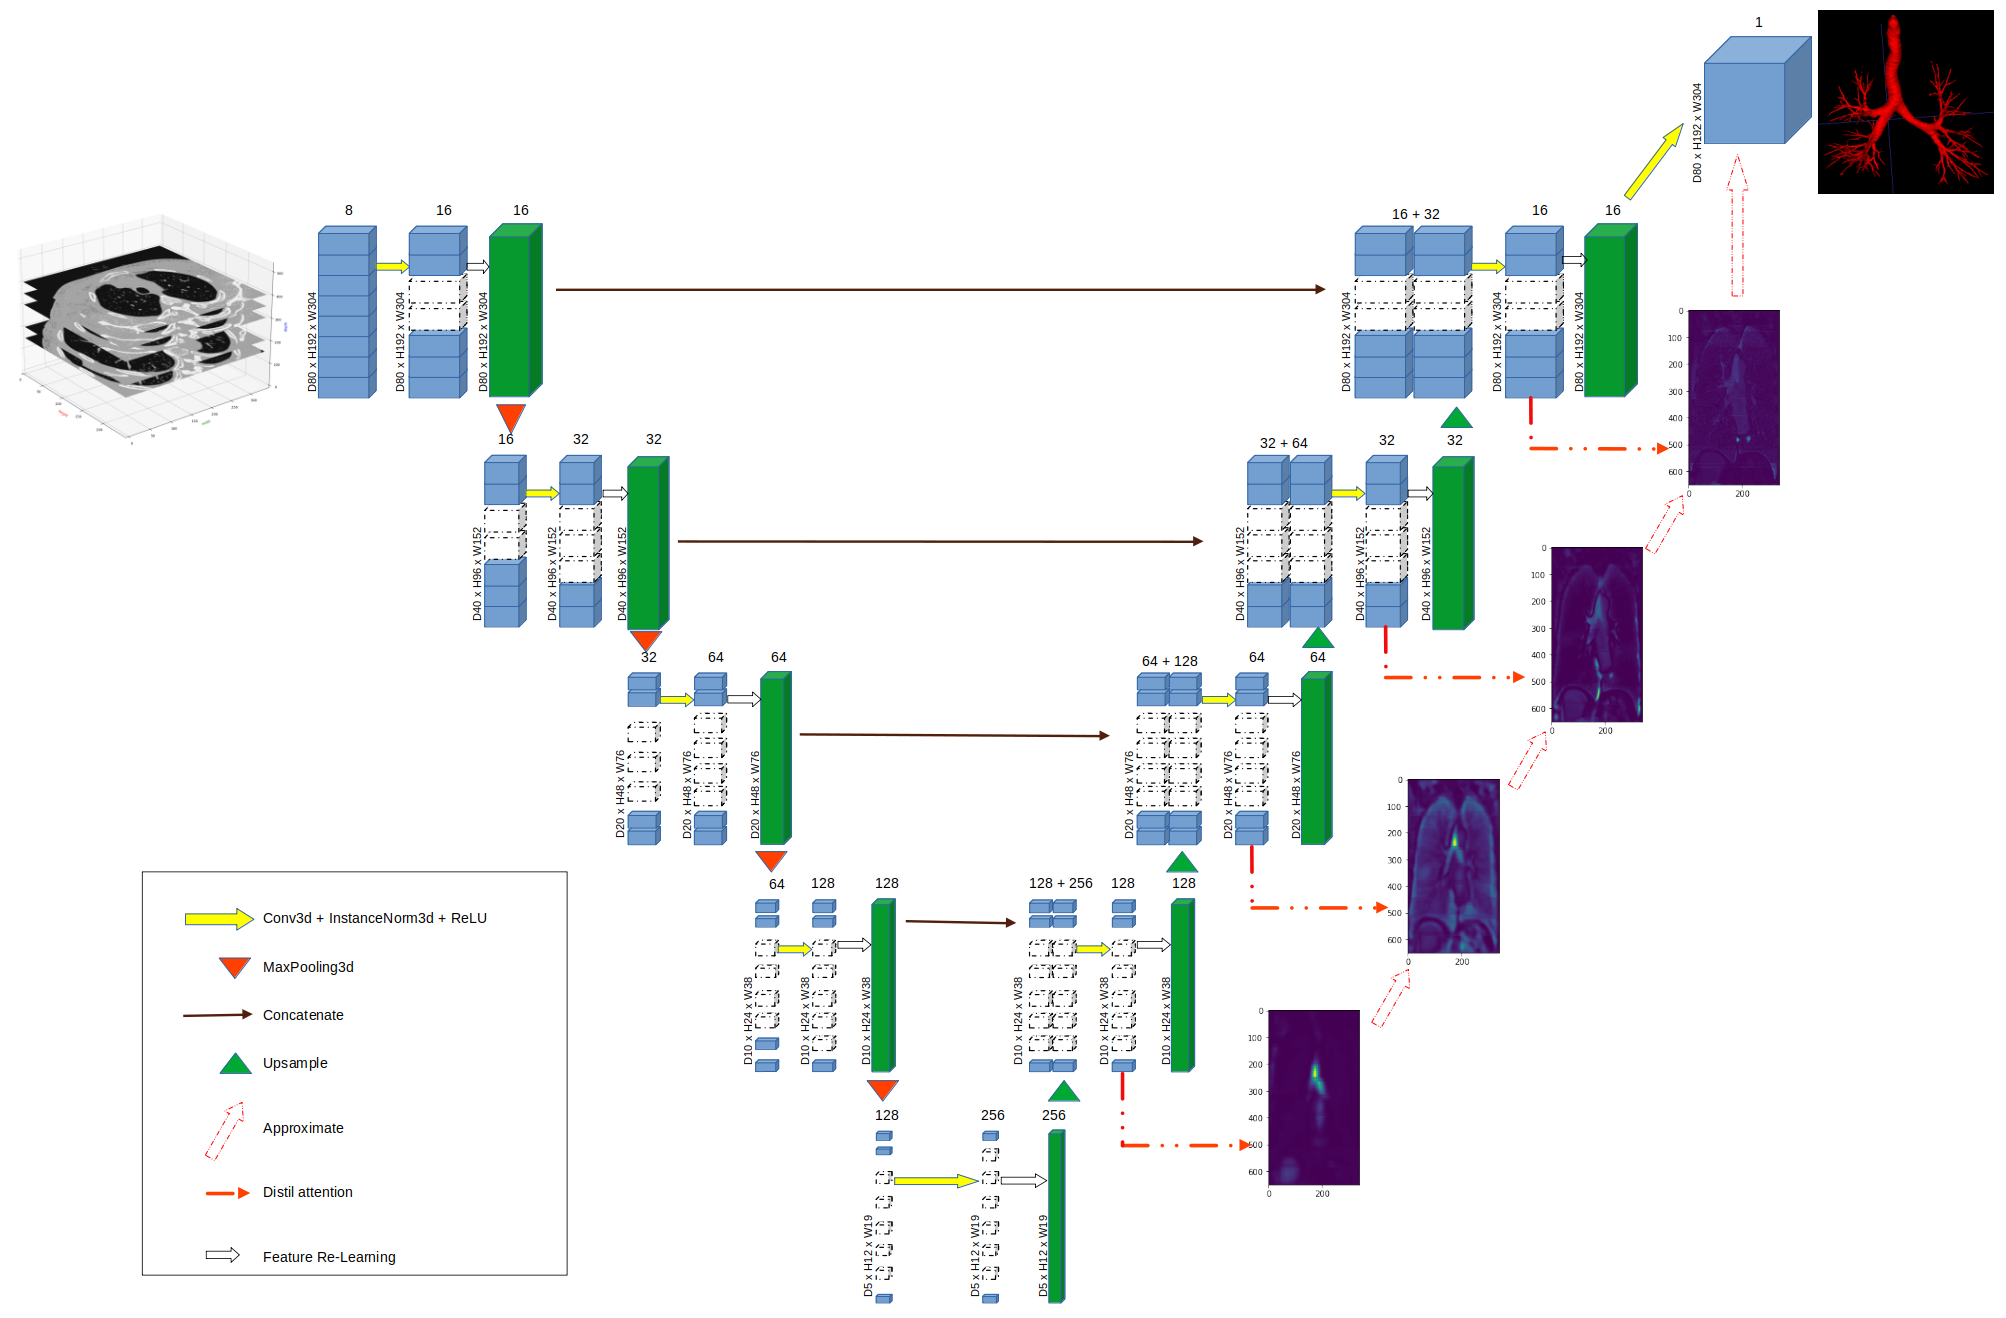
\includegraphics[width=0.95\textheight, height=\textwidth, angle=90]{Baseline_AD_FRL}
    \bicaption[3D-UNet + Attention Distillation + Feature Re-Learning网络结构示意图]
        {3D-UNet + Attention Distillation + Feature Re-Learning网络结构示意图}
        {The architecture of 3D-UNet + Attention Distillation + Feature Re-Learning network}
    \label{fig:3dunet_ad_fr}
\end{figure}
需要说明的是,特征再学习模块并没有改变特征的维数,依然保持与同一级的卷积层块的特征相同的Shape。因此,3D-UNet网络继续按照原来的方式工作。
通道级的特征再学习模块将卷积层特征的通道先压缩再恢复,将多个通道进行重组。这样,有信息性的通道得到加强,而无信息性的通道就被抑制削弱,分割的
性能得到提升。

图\ref{fig:3dunet_ad_fr}的网络结构也是我们最终的网络结构模型,在3D-UNet网络基准模型的基础上加上我们所做的两个改进模块:通道级的特征再学习模块
和注意力蒸馏模块。我们称这个新的网络结构为3D-UNet + Attention Distillation + Feature Re-Learning,简写为3D-UNet + AD + FRL网络结构。

\section{综合实验}

有了前述两章对3D-UNet网络基准模型的改进,我们得到了最终的改进的网络模型3D-UNet + AD + FRL。现在我们来做一次对比实验,也是最终的综合性实验,看看
支气管气道树最终的分割效果如何,综合评估分割模型的性能表现。

我们还是采用跟\ref{sec:baseline_experiment_training}节的3D-UNet网络基准模型的实验同样的训练集、验证集、测试集的数据,相同的实验条件。
我们在上海交通大学高性能计算中心的AI超算上使用了8块NVIDIA Tesla V100显卡来同时进行训练,开启了8个进程,设置Batch-Size=8,训练了60个迭代周期,
验证和测试各1个迭代周期,整个实验耗时39小时22分钟。

集中验证集和测试集,计算它们的评价指标数据,如表\ref{tbl:comprehensive_metrics_overview}所示。
\begin{table}[ht]
    \centering
    \bicaption[综合实验验证集和测试集的评价指标一览]
        {综合实验验证集和测试集的评价指标一览\\每一项指标栏用双下划线加粗黑体标示出表现最优秀的, 用波浪线标示出表现最差的.}
        {The metrics overview of comprehensive experiment for valset and testset}
    \label{tbl:comprehensive_metrics_overview}
    \begin{tabular}{cccccccc}
        \toprule
                       & FPR            & FNR            & Sensitivity    & Precision      & DSC            & BD             & TLD            \\
        \midrule
        ATM\_001\_0000 & \uuline{{\bf 0.006}} & 7.119          & 92.88          & \uuline{{\bf 98.18}} & 95.04          & \uwave{66.84}  & 82.96          \\
        ATM\_024\_0000 & 0.031          & \uwave{7.676}  & \uwave{92.32}  & 91.01          & 91.66          & 84.18          & 92.28          \\
      % ATM\_029\_0000 & 0.022          & 9.337          & 90.66          & 91.09          & 90.88          & 76.92          & 87.08          \\
        ATM\_034\_0000 & 0.023          & 3.712          & 96.29          & 96.00          & 96.06          & 88.44          & 93.92          \\
        ATM\_041\_0000 & 0.046          & 4.59           & 95.41          & 87.19          & 90.65          & 79.27          & 88.92          \\
        ATM\_054\_0000 & 0.031          & 4.924          & 95.08          & 92.47          & 93.76          & 70.28          & \uwave{82.27}  \\
        ATM\_055\_0000 & 0.035          & 4.141          & 95.86          & 91.31          & 93.24          & 80.72          & 88.63          \\
        ATM\_057\_0000 & 0.034          & 5.475          & 94.53          & 91.42          & 92.94          & 74.57          & 85.34          \\
        ATM\_060\_0000 & 0.023          & 3.4            & 96.6           & 93.67          & 94.96          & 83.76          & 90.9           \\
        ATM\_061\_0000 & 0.027          & 4.291          & 95.71          & 92.16          & 93.62          & 79.23          & 88.00          \\
        ATM\_074\_0000 & 0.055          & 3.997          & 96.00          & 86.13          & 90.8           & 82.23          & 89.15          \\
        ATM\_075\_0000 & 0.024          & 5.497          & 94.5           & 93.15          & 93.76          & 77.36          & 86.64          \\
        ATM\_080\_0000 & 0.03           & 4.487          & 95.51          & 92.27          & 93.86          & 76.57          & 88.32          \\
        ATM\_091\_0000 & 0.042          & 4.036          & 95.96          & 89.15          & 92.43          & 75.53          & 87.34          \\
        ATM\_150\_0000 & \uwave{0.084}  & 3.823          & 96.18          & \uwave{79.61}  & \uwave{87.11}  & 70.35          & 87.09          \\
        ATM\_158\_0000 & 0.043          & 3.584          & 96.42          & 87.12          & 91.53          & 78.66          & 89.93          \\
        ATM\_163\_0000 & 0.034          & 4.417          & 95.58          & 92.17          & 93.85          & 78.39          & 90.1           \\
      % ATM\_174\_0000 & 0.031          & 14.06          & 85.94          & 94.82          & 88.87          & 41.9           & 55.07          \\
      % ATM\_197\_0000 & 0.027          & 9.032          & 90.97          & 92.05          & 91.04          & 54.68          & 76.59          \\
      % ATM\_215\_0000 & 0.02           & 10.59          & 89.41          & 92.67          & 91.01          & 65.97          & 80.35          \\
        ATM\_245\_0000 & 0.036          & 0.401          & \uuline{{\bf 99.6}}  & 84.2           & 91.26          & \uuline{{\bf 100}}   & 99.89          \\
        ATM\_246\_0000 & 0.039          & \uuline{{\bf 0.288}} & 99.39          & 82.94          & 90.42          & \uuline{{\bf 100}}   & \uuline{{\bf 99.9}}  \\
        ATM\_260\_0000 & 0.017          & 0.984          & 99.02          & 94.59          & \uuline{{\bf 96.57}} & 97.24          & 96.57          \\
        ATM\_266\_0000 & 0.018          & 2.352          & 97.65          & 93.35          & 95.33          & 96.89          & 96             \\
        ATM\_271\_0000 & 0.046          & 1.354          & 98.65          & 87.13          & 92.45          & 96             & 95.64          \\
      % ATM\_505\_0000 & 0.036          & 37.12          & 62.88          & 88.98          & 73.24          & 29.23          & 47.34          \\
        ATM\_638\_0000 & 0.014          & 3.294          & 96.71          & 95.3           & 96.26          & 91.16          & 95.2           \\
        ATM\_688\_0000 & 0.016          & 2.107          & 97.89          & 94.49          & 95.36          & 91.77          & 95.32          \\
        \midrule
        平均值          & 0.0328         & 3.737          & 96.249         & 90.653         & 93.171         & 83.454         & 90.883         \\
        \bottomrule
    \end{tabular}
\end{table}
在每一项指标上用双下划线加粗黑体标示出表现最优秀的,用波浪线标示出最差的。并在最后一行计算出每个指标的平均值,以作为参考。

我们从表\ref{tbl:comprehensive_metrics_overview}挑选出9个有代表性的病例来显示支气管气道树三维模型,见图\ref{fig:airway_segmentation_overview}。
%\begin{table}[!ht]
%    \centering
%    \bicaption[综合实验验证集和测试集的气道树分割效果一览]
%        {综合实验验证集和测试集的气道树分割效果一览}
%        {The airway tree segmentation overview of comprehensive experiment for valset and testset}
%    \label{fig:airway_segmentation_overview}
%    \begin{tabular}{|c|c|c|}
%        \hline
%        ATM\_260\_0000 & ATM\_266\_0000 & ATM\_638\_0000 \\
%        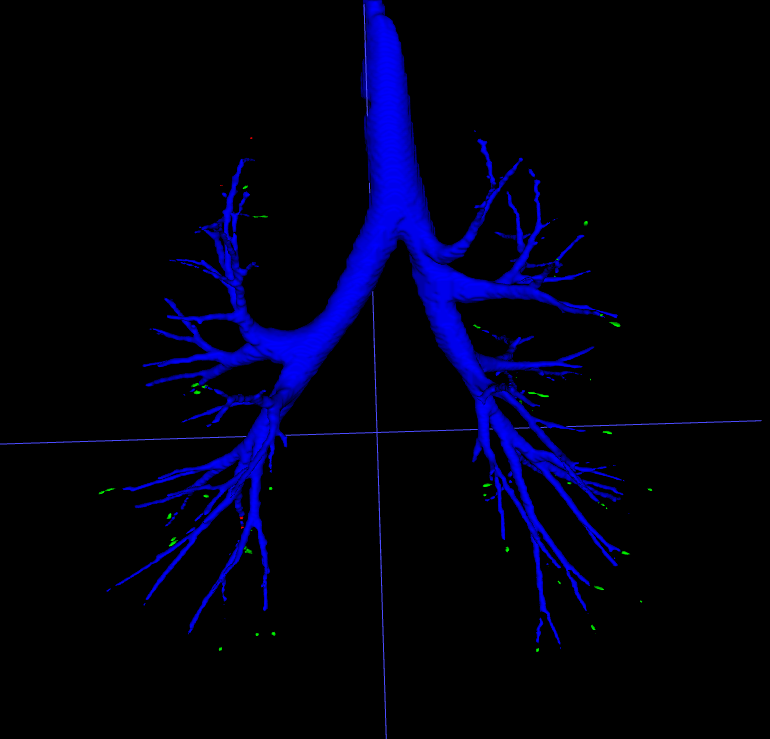
\includegraphics[width=0.3\textwidth]{results/baseline_fr_ds_ad/val_test/ATM_260_0000_airway_tree_with_3colors_at_test_epoch1} &
%        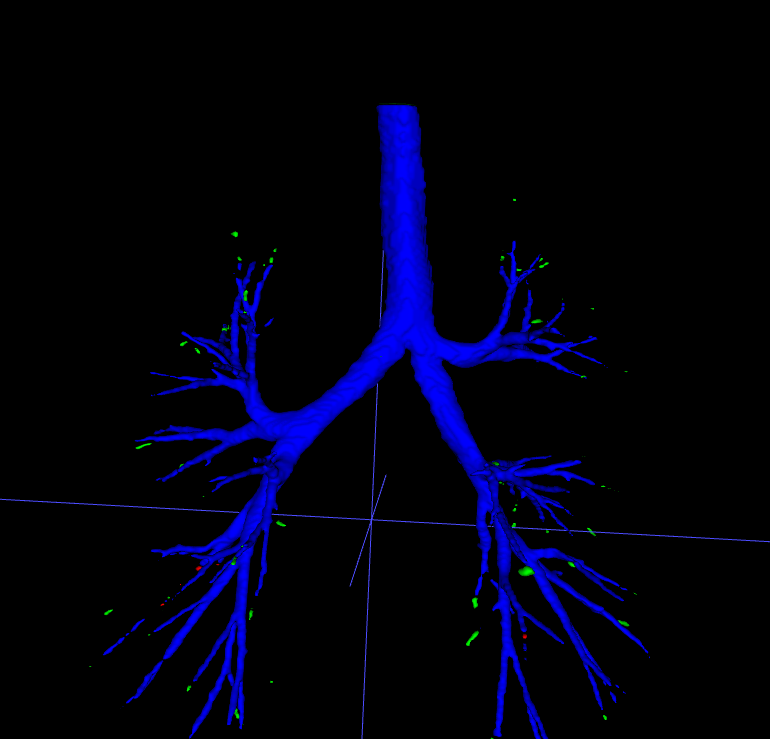
\includegraphics[width=0.3\textwidth]{results/baseline_fr_ds_ad/val_test/ATM_266_0000_airway_tree_with_3colors_at_test_epoch1} &
%        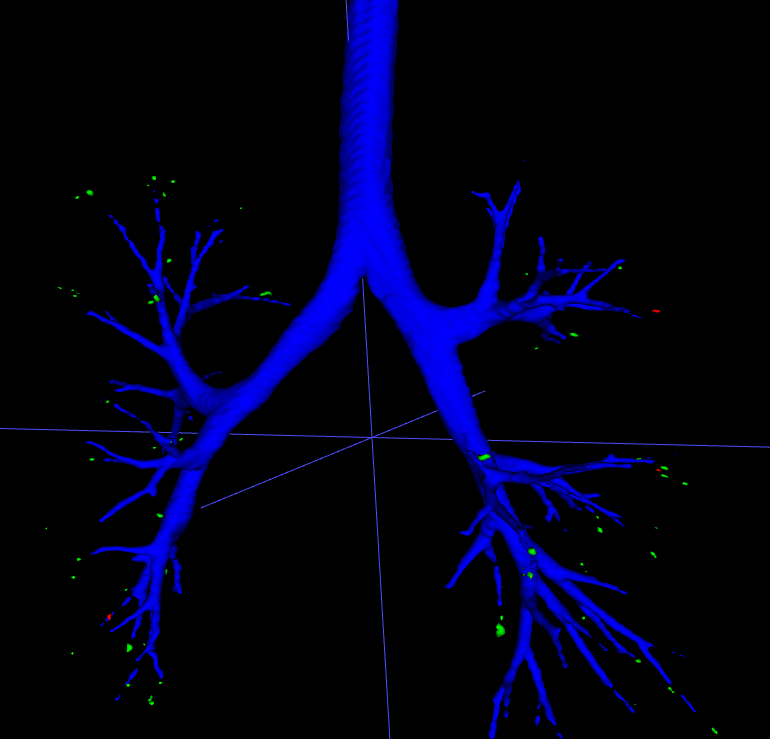
\includegraphics[width=0.3\textwidth]{results/baseline_fr_ds_ad/val_test/ATM_638_0000_airway_tree_with_3colors_at_test_epoch1} \\
%        \hline
%        ATM\_055\_0000 & ATM\_060\_0000 & ATM\_075\_0000 \\
%        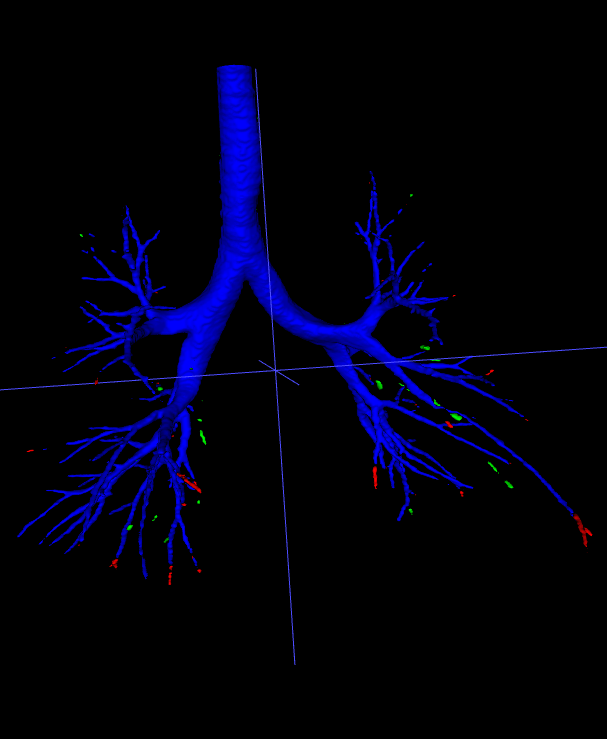
\includegraphics[width=0.3\textwidth]{results/baseline_fr_ds_ad/val_test/ATM_055_0000_airway_tree_with_3colors_at_val_epoch1} &
%        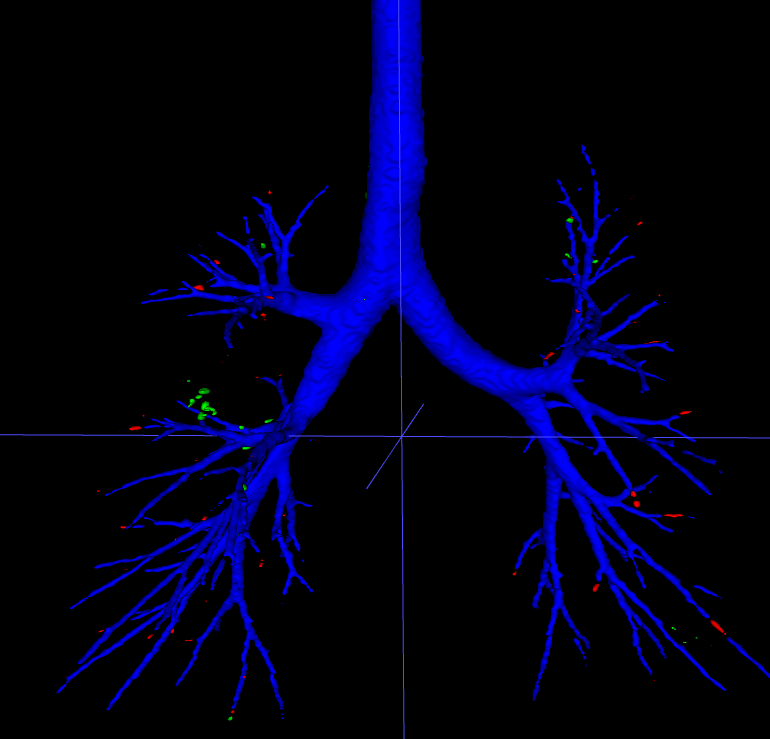
\includegraphics[width=0.3\textwidth]{results/baseline_fr_ds_ad/val_test/ATM_060_0000_airway_tree_with_3colors_at_test_epoch1} &
%        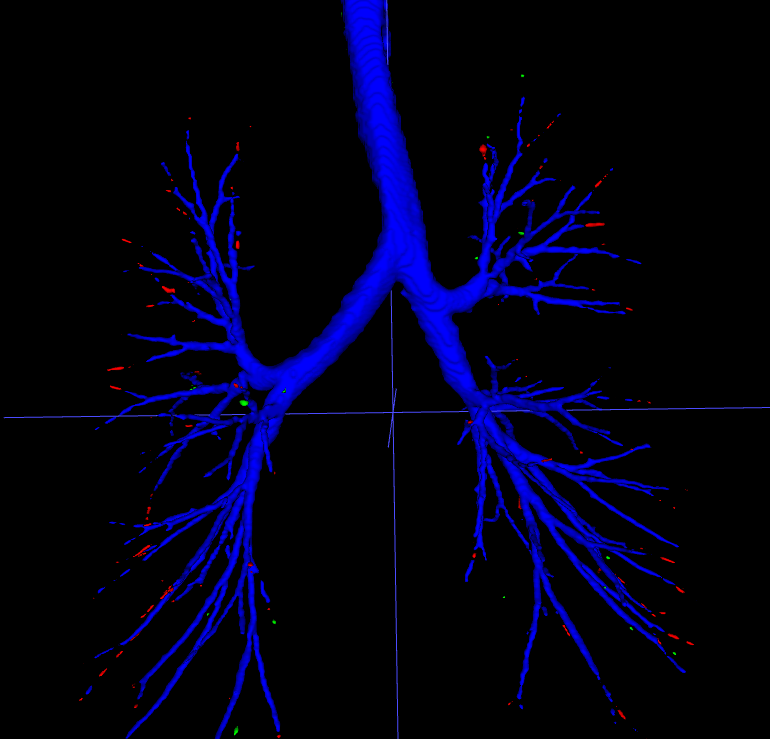
\includegraphics[width=0.3\textwidth]{results/baseline_fr_ds_ad/val_test/ATM_075_0000_airway_tree_with_3colors_at_test_epoch1} \\
%        \hline
%        ATM\_271\_0000 & ATM\_061\_0000 & ATM\_074\_0000 \\
%        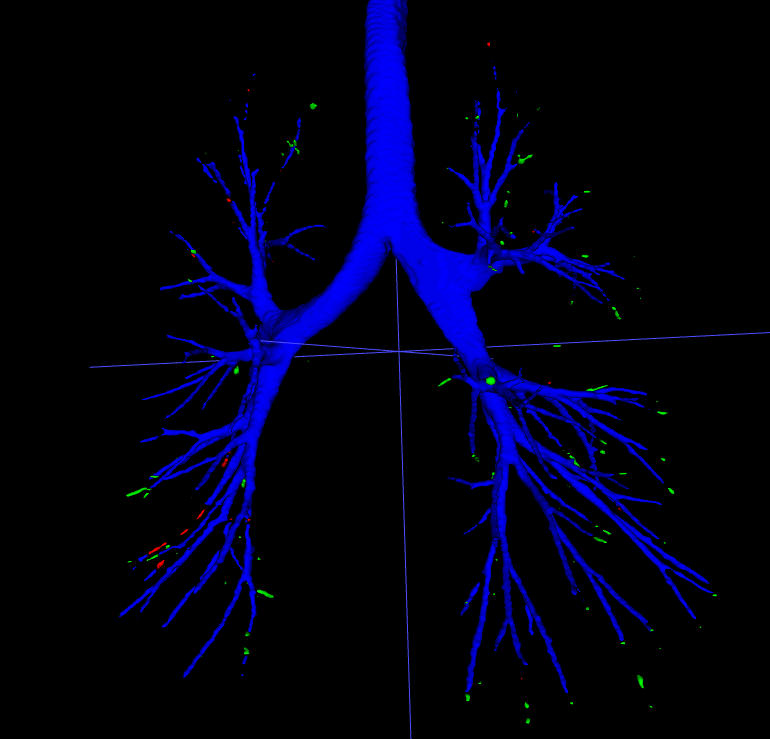
\includegraphics[width=0.3\textwidth]{results/baseline_fr_ds_ad/val_test/ATM_271_0000_airway_tree_with_3colors_at_test_epoch1} &
%        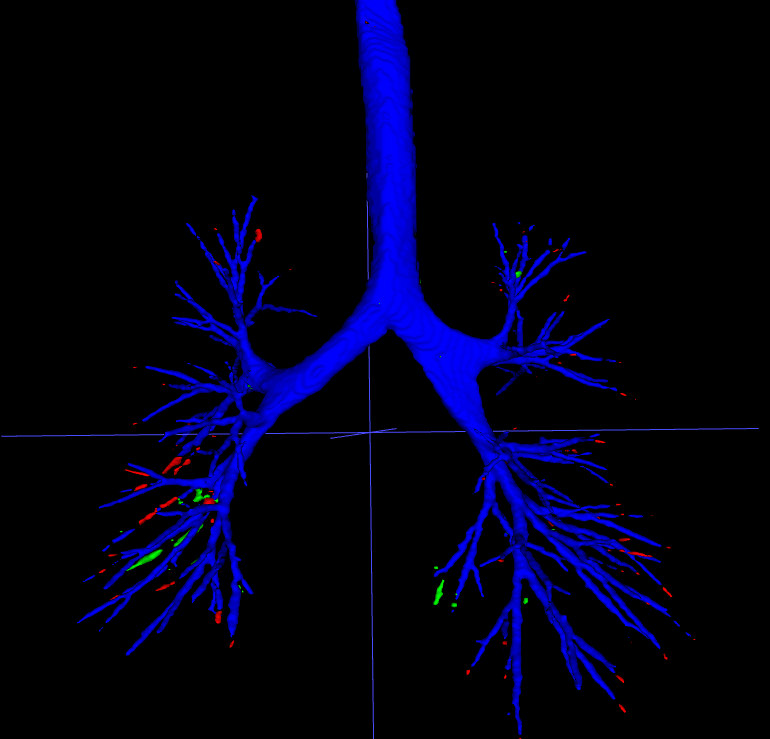
\includegraphics[width=0.3\textwidth]{results/baseline_fr_ds_ad/val_test/ATM_061_0000_airway_tree_with_3colors_at_test_epoch1} &
%        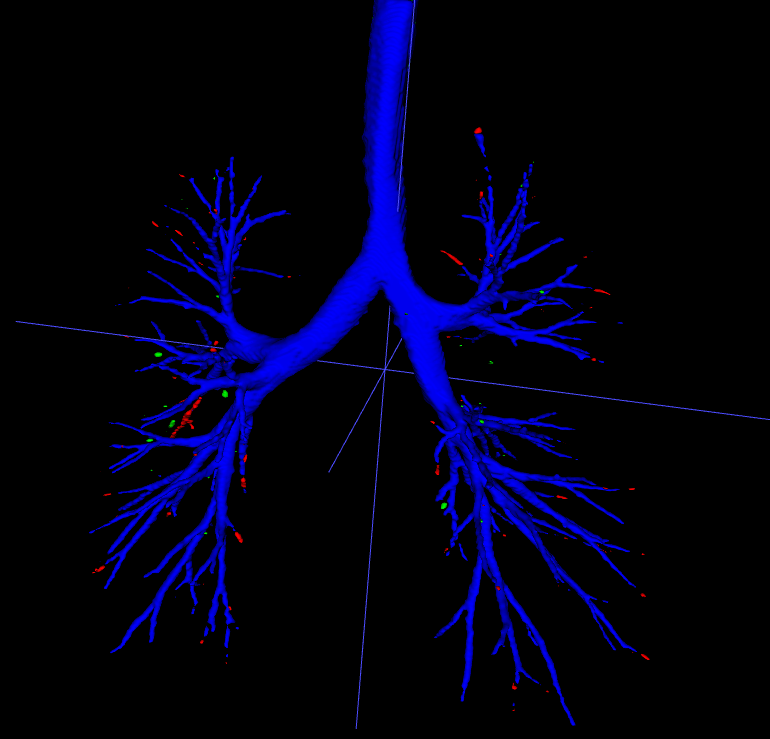
\includegraphics[width=0.3\textwidth]{results/baseline_fr_ds_ad/val_test/ATM_074_0000_airway_tree_with_3colors_at_test_epoch1} \\
%        \hline
%    \end{tabular}
%\end{table}

\begin{figure}[!ht]
	\centering
	\begin{subfigure}{0.325\textwidth}
		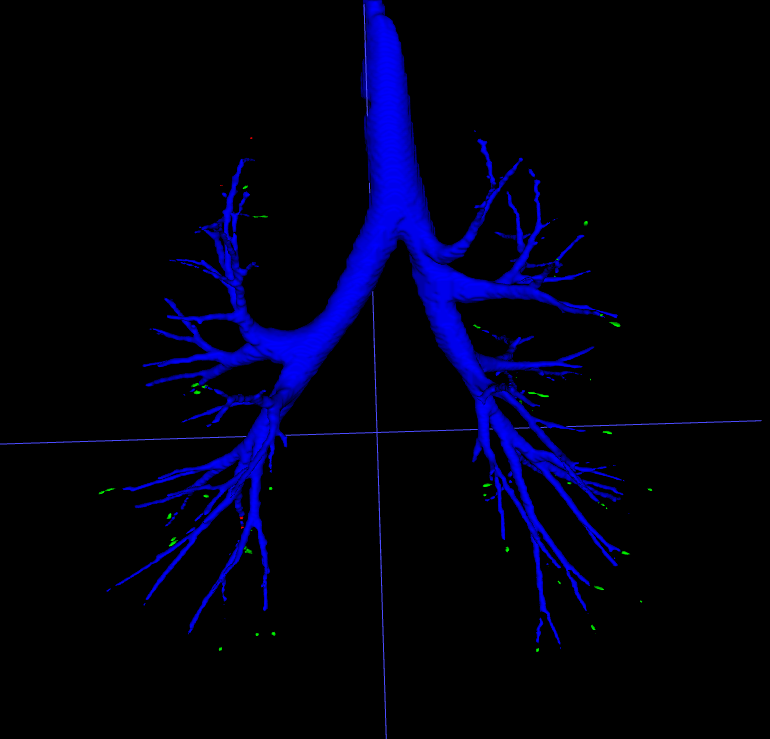
\includegraphics[width=\textwidth]{results/baseline_fr_ds_ad/val_test/ATM_260_0000_airway_tree_with_3colors_at_test_epoch1}
		\caption{ATM\_260\_0000}
	\end{subfigure}
	\hfill
	\begin{subfigure}{0.325\textwidth}
		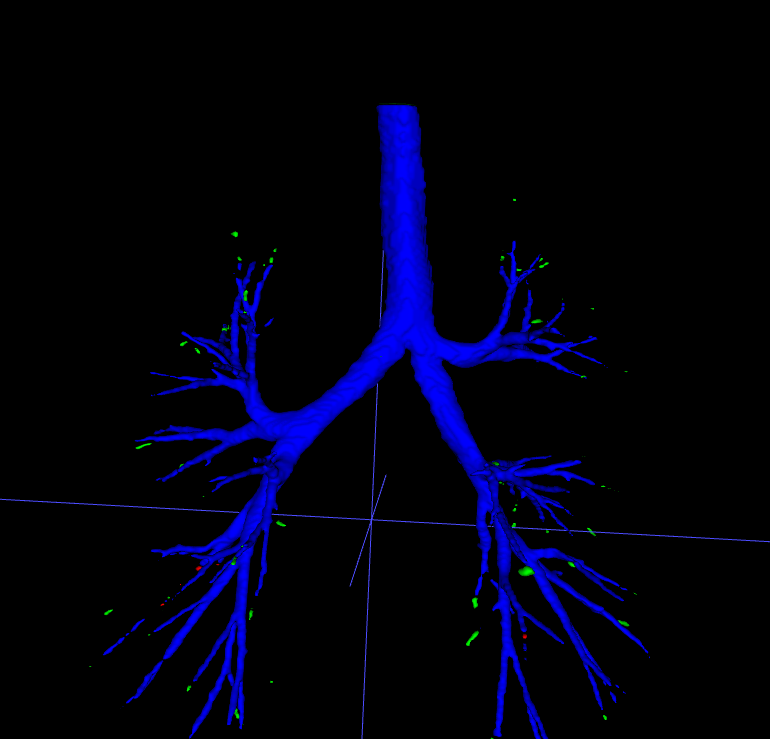
\includegraphics[width=\textwidth]{results/baseline_fr_ds_ad/val_test/ATM_266_0000_airway_tree_with_3colors_at_test_epoch1}
		\caption{ATM\_266\_0000}
	\end{subfigure}
	\hfill
	\begin{subfigure}{0.325\textwidth}
		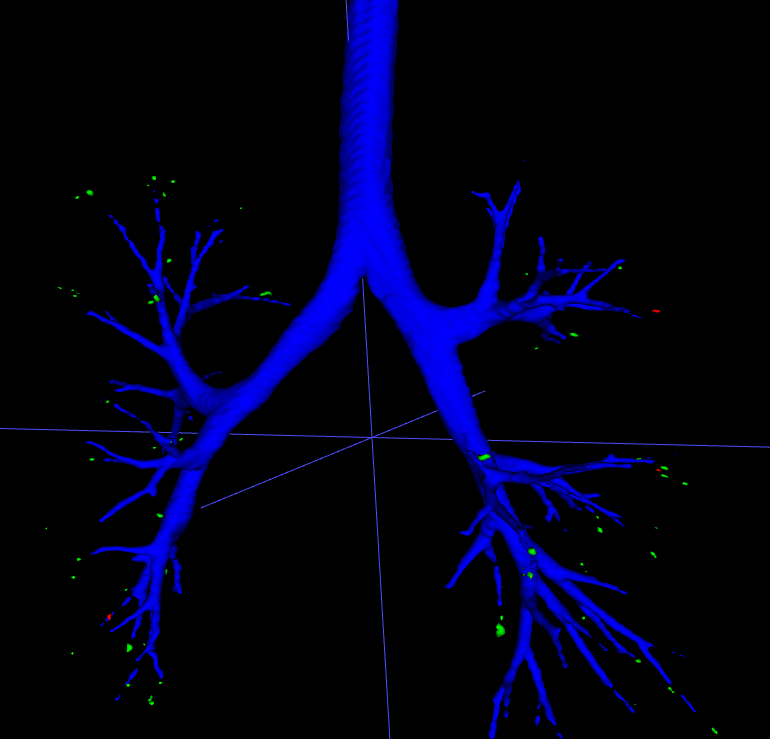
\includegraphics[width=\textwidth]{results/baseline_fr_ds_ad/val_test/ATM_638_0000_airway_tree_with_3colors_at_test_epoch1}
		\caption{ATM\_638\_0000}
	\end{subfigure}
	\\
	\begin{subfigure}{0.325\textwidth}
		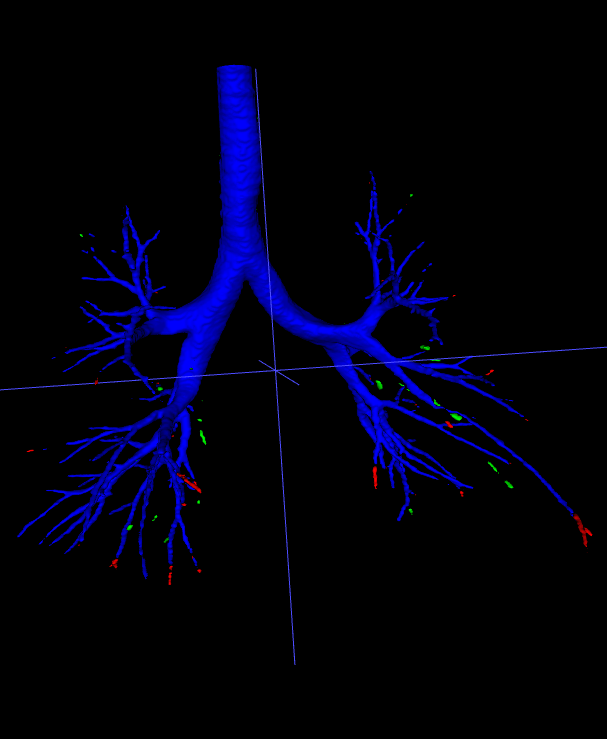
\includegraphics[width=\textwidth]{results/baseline_fr_ds_ad/val_test/ATM_055_0000_airway_tree_with_3colors_at_val_epoch1}
		\caption{ATM\_055\_0000}
	\end{subfigure}
	\hfill
	\begin{subfigure}{0.325\textwidth}
		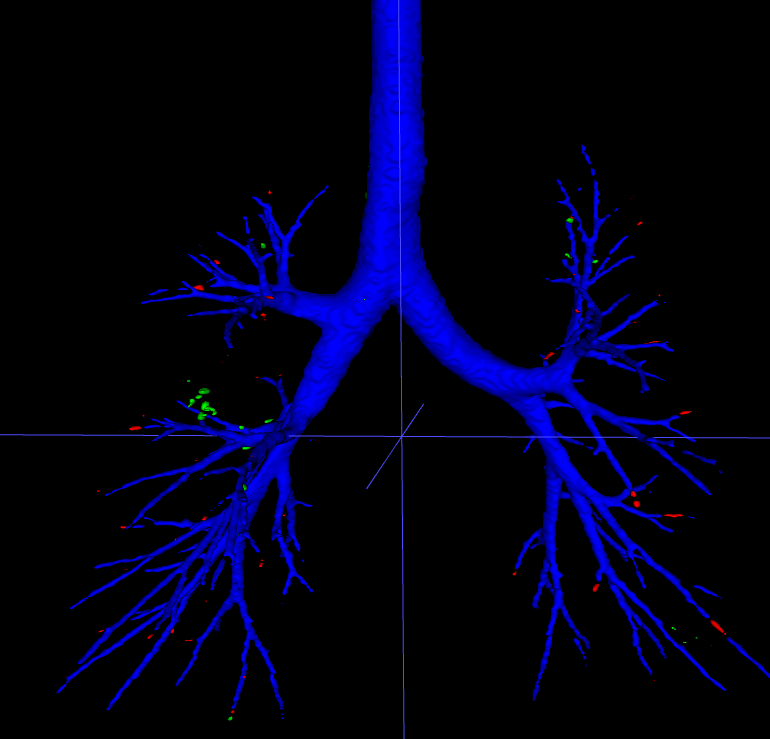
\includegraphics[width=\textwidth]{results/baseline_fr_ds_ad/val_test/ATM_060_0000_airway_tree_with_3colors_at_test_epoch1}
		\caption{ATM\_060\_0000}
	\end{subfigure}
	\hfill
	\begin{subfigure}{0.325\textwidth}
		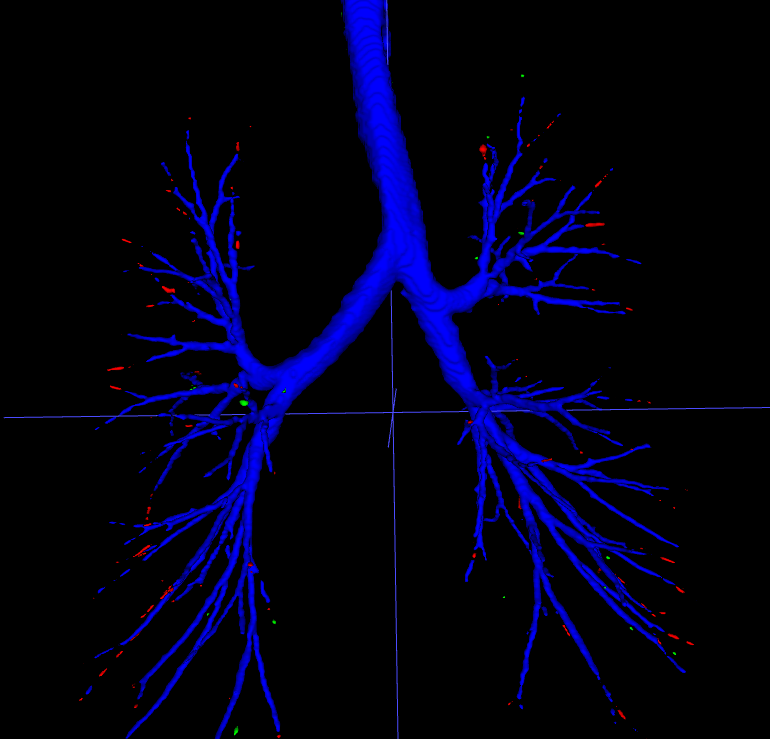
\includegraphics[width=\textwidth]{results/baseline_fr_ds_ad/val_test/ATM_075_0000_airway_tree_with_3colors_at_test_epoch1}
		\caption{ATM\_075\_0000}
	\end{subfigure}
	\\
	\begin{subfigure}{0.325\textwidth}
		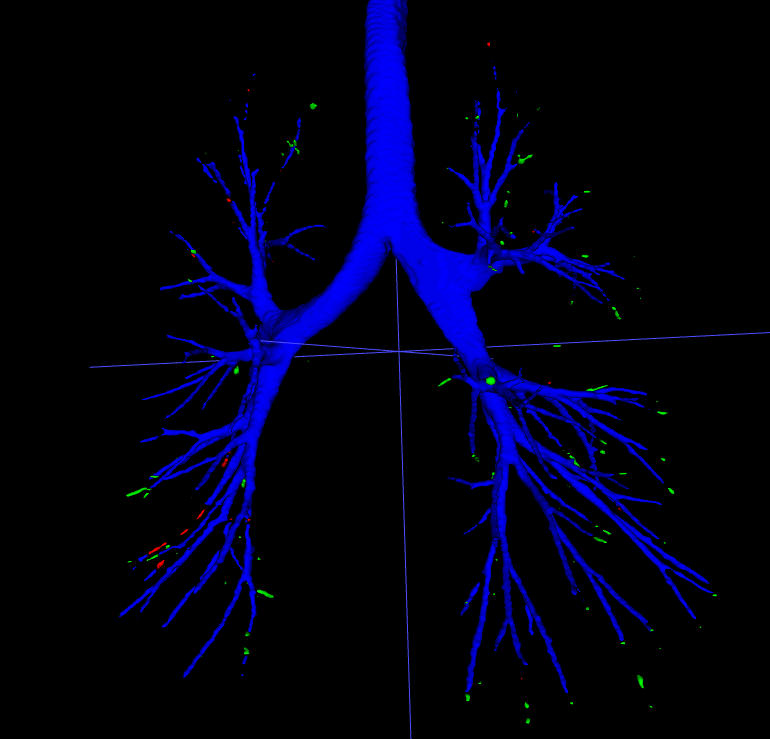
\includegraphics[width=\textwidth]{results/baseline_fr_ds_ad/val_test/ATM_271_0000_airway_tree_with_3colors_at_test_epoch1}
		\caption{ATM\_271\_0000}
	\end{subfigure}
	\hfill
	\begin{subfigure}{0.325\textwidth}
		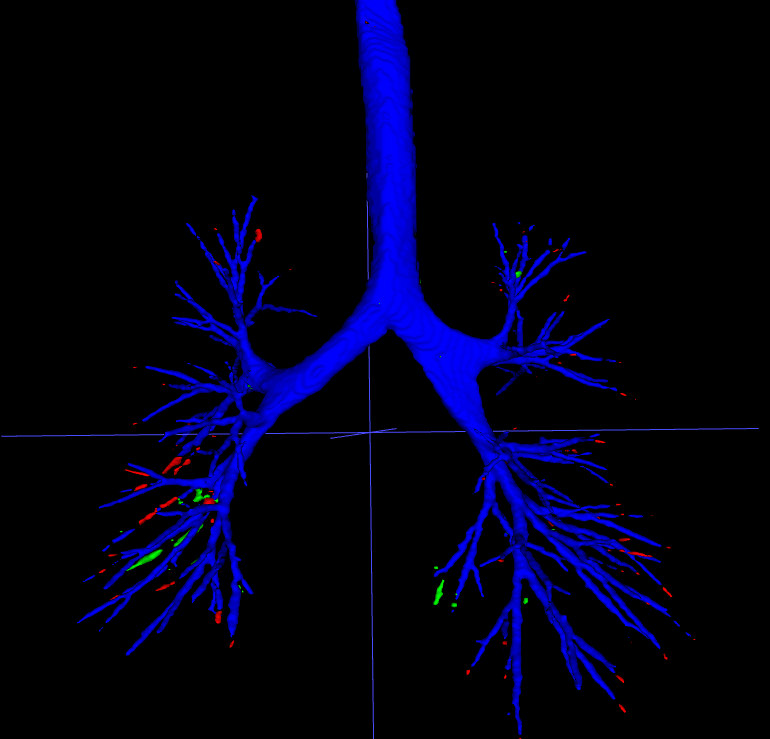
\includegraphics[width=\textwidth]{results/baseline_fr_ds_ad/val_test/ATM_061_0000_airway_tree_with_3colors_at_test_epoch1}
		\caption{ATM\_061\_0000}
	\end{subfigure}
	\hfill
	\begin{subfigure}{0.325\textwidth}
		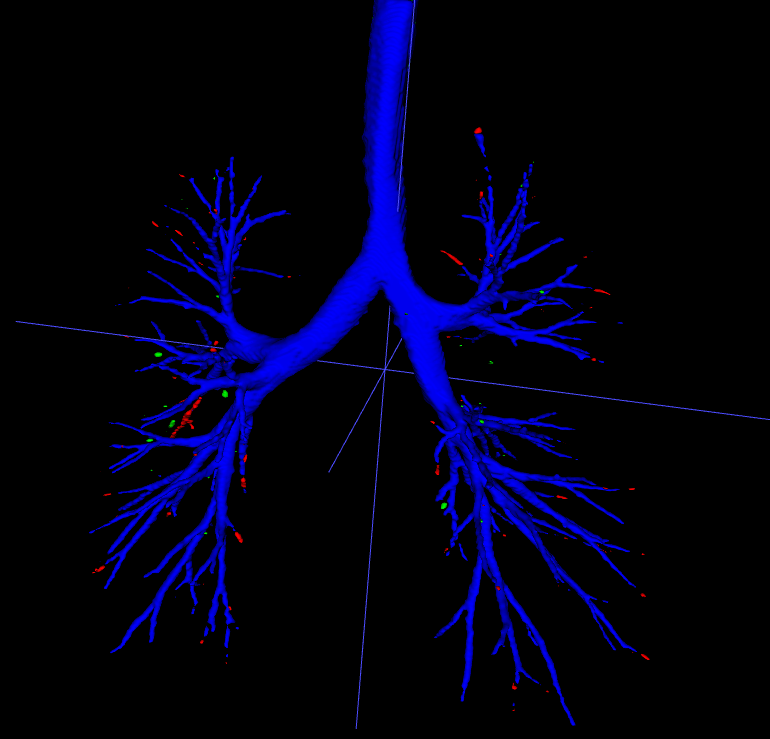
\includegraphics[width=\textwidth]{results/baseline_fr_ds_ad/val_test/ATM_074_0000_airway_tree_with_3colors_at_test_epoch1}
		\caption{ATM\_074\_0000}
	\end{subfigure}
	\bicaption[综合实验验证集和测试集的气道树分割效果一览]
        {综合实验验证集和测试集的气道树分割效果一览}
        {The airway tree segmentation overview of comprehensive experiment for valset and testset}
    \label{fig:airway_segmentation_overview}
\end{figure}
可以看到,末梢支气管的分割比之前的两个实验的效果要好得多,虽然不能完全排除红色假阴性(漏检)体素和绿色假阳性(误检)体素,总体上将末梢支气管这些精细特征都给分割
出来了,说明通道级特征再学习的改进方法提高了3D-UNet + AD + FRL网络模型的性能。当然这些改善是注意力蒸馏Attention Distillation和通道级特征再学习
Channel-wise Feature Re-Learning两个改进功能共同作用的,单一的改进还达不到这样的效果。


\section{性能指标对比}

完成了综合实验之后,我们就性能指标与一些经典的网络结构进行对比。我们选择了V-Net\cite{Milletar2016VNetFC}, VoxResNet\cite{CHEN2018446}和
Attention-Gated U-Net\cite{Oktay2018AttentionUL}来比较FPR、DSC、BD和TLD四个指标。我们也跟State-of-the-art(SOTA)的几个方法,诸如Wang Chenglong
等人\cite{Wang2019TubularSegment}提出的使用空间全连接网络解决管状结构的分割问题, Antonio Juarez等人提出一个3D-UNet + GNN联合型
网络\cite{Juarez2019Joint3DUNetGraph}用于支气管气道树的分割,Qin Yulei等人\cite{Qin2019AirwayNet}提出一个体素连接的AirwayNet方法解决精确的
气道树分割,Antonio Juarez等人\cite{Juarez2018AutoAirwaySegment}较早提出的应用3D-UNet网络用于支气管气道树分割,还有Dakai Jin等
人\cite{Dakai2017GraphRefinement}则是结合3D CNN与Graph Refinement在一个不完整标注的数据集上做的气道树分割,进行比较。我们选取FPR、DSC、BD和TLD指标
的平均值来跟它们比较,见表\ref{tbl:metrics_comparison_table}。
\begin{table}[ht]
    \centering
    \bicaption[性能指标比较表]
        {性能指标比较表}
        {The comparison table of performance metrics}
    \label{tbl:metrics_comparison_table}
    \begin{tabular}{l|c|cccc}
        \hline
        \multicolumn{2}{c|}{方法}     & FPR (\%) & DSC (\%) & BD (\%) & TLD (\%) \\
        \hline
        \multicolumn{2}{c|}{\makecell{我们的方法\\3D-UNet + AD + FRL}} & 0.0328 & 93.171 & 83.454 & \uuline{\bf 90.883} \\
        \hline
        \hline
        \multirow{3}*{\makecell{经典的\\网络}} & V-Net\cite{Milletar2016VNetFC} & 0.024 & 92.1 & 91.0 & 81.6 \\
        
                                             & VoxResNet\cite{CHEN2018446} & 0.012 & 92.7 & 88.2 & 76.4 \\
        
                                             & Attention-Gated U-Net\cite{Oktay2018AttentionUL} & 0.031 & 92.5 & \uuline{\bf 93.8} & 88.2 \\
        
        \hline
        \hline
        \multirow{5}*{\makecell{SOTA\\的\\方\\法}} & \makecell{Wang Chenglong等人\cite{Wang2019TubularSegment}\\提出的空间全连接网络} & 0.018 & 93.5 & 93.4 & 85.6 \\
        
        \cline{2-2}  & \makecell{Antonio Juarez等人\cite{Juarez2019Joint3DUNetGraph}\\提出的3D-UNet + GNN\\联合型网络} & \uuline{\bf 0.009} & 87.5 & 77.5 & 66.0 \\

						\cline{2-2}  & \makecell{Qin Yulei等人\cite{Qin2019AirwayNet}\\提出的体素连接\\的AirwayNet网络} & 0.014 & \uuline{\bf 93.7} & 91.6  & 82.1 \\
        
        \cline{2-2} & \makecell{Antonio Juarez等人\cite{Juarez2018AutoAirwaySegment}\\较早提出的应用3D-UNet\\用于气道树分割的方法} & 0.014 & 93.6 & 91.9 & 80.7 \\
        
        \cline{2-2} & \makecell{Dakai Jin等人\cite{Dakai2017GraphRefinement}提出的\\结合3D CNN与Graph \\Refinement的方法} & 0.017 & 93.6 & 93.1 & 84.8 \\
        \hline
        \hline
        \multicolumn{2}{c|}{\makecell{我们的方法在一些病例\\上取得的优秀表现\\以ATM\_260\_0000为例}} & 0.017 & \uuline\bf 96.57 & 97.24 & 96.57 \\
        \hline
    \end{tabular}
\end{table}
可以看出,在DSC和TLD两项指标上,我们的方法要比经典的网络的方法要优秀一些,但跟SOTA的方法比,FPR、DSC和BD三项指标都比较落后,只有TLD一项指标还保持着领先。
当然,我们也在一些病例上取得了很优秀的结果。


\section{本章小结}

本章针对末梢支气管这样的精细特征引入了特征再学习功能。我们认为在不同的空间位置,特征应该具有不同的重要性。在枝干支气管这样的粗糙特征处赋予一般的权重,在末梢支气管
这样的精细特征处应该赋予比较高的权重,而对于没有没有特征的背景或角落处则应该逐渐降低其权重。正是基于这样的一个想法,我们就想在卷积层块之后,最大池化层之前引入一种
新的方法来调整特征的权重,从而想捕获更精细的特征。这种新方法就是通道级特征再学习(Channel-wise Feature Re-Learning, FRL)方法。

我们详细介绍了通道级特征再学习方法的基本原理,提出了汇聚特征的计算公式。其中最重要的是特征立方体(见图\ref{fig:spatial_integration})的体积分过程,将体积分拆分
为沿着$Depth$方向、$Height$方向、$Width$方向分别进行积分。这种积分是将特征立方体$\mathbbm{Feat}_m$从$D \times H \times W$大小挤压成$1 \times 1 \times W$,
$1 \times H \times 1$和$D \times 1 \times 1$的形状。这种挤压过程实际上是两次累积求和过程,它是借鉴了注意力蒸馏(见图\ref{fig:attention_distillation})
的思想,就是想在空间的三个维度上都各自产生聚焦。将这三个方向的积分加起来(见式\ref{eq:sum_of_3integrations})后,为了将多个通道重新组合,加强有信息的通道,抑制
无信息的通道,我们又设计了一个降通道的卷积层和恢复原通道数的卷积层。两个卷积层用来处理三个方向的积分之和的数据得到$\varPsi\left(\mathbbm{Feat}_m\right)$
(见\ref{eq:features_element_wise_multiply}式),其跟卷积层输出的特征$\mathbbm{Feat}_m$在维数上是一样的,都是$B \times C \times D \times H \times W$的大小,
这样我们就可以进行逐元素相乘。从图\ref{fig:feature_dimensions}、图\ref{fig:spatial_integration}, 公式\ref{eq:feature_dimensions}到公式
\ref{eq:features_element_wise_multiply}是特征再学习的完整计算过程。特征再学习方法起的作用是在训练过程中、重要的气道特征随着特征再学习模块所赋予的新权重而
逐渐被重视,而无关的区域则随着权重的降低而慢慢被忽略。

了解了通道级特征再学习的原理、计算过程和作用后,我们对3D-UNet网络基准基准模型进行改进,引入特征再学习模块,将其插入在每一层的卷积层块之后和最大池化层之间,
见图\ref{fig:3dunet_ad_fr}中的绿色柱体。使用Python实现了这个改进的3D-UNet + Attention Distillation + Feature Re-Learning网络之后,我们进行了一次综合
实验。实验结果表明注意力蒸馏模块和特征再学习模块明显帮助提高了模型的性能,从表\ref{fig:airway_segmentation_overview}看到分割出来的三维气道树模型表现为很完整
的一棵树,枝干支气管和末梢支气管都已经完整分割出来。

完成综合实验,我们还做了指标对比研究。将我们的方法与经典的网络V-Net, VoxResNet和Attention-Gated U-Net比较FPR、DSC、BD、TLD四个指标,
在DSC与TLD两项指标上取得领先。我们也跟State-of-the-art (SOTA)的方法进行对比,虽然在TLD指标上取得明显领先,但在FPR、BD两项指标确实明显落后。当然,我们的
方法也在一些病例上取得了优秀的表现。

至此,本论文完成所有的研究与实验。